\documentclass{article}

\usepackage[letterpaper, margin=1in]{geometry}

\usepackage{amsmath}
\usepackage{amssymb}
\usepackage{amsbsy}
\usepackage{graphicx}
\usepackage{caption}
\usepackage{subcaption}
\usepackage{multirow}
\usepackage{placeins}

\graphicspath{{../images/}}

\let\bld\boldsymbol

\usepackage[backend=bibtex]{biblatex}
\bibliography{../hyparticle}

\author{Aditya Kashi}
\date{December 23, 2016}
\title{Numerical Analysis Project Report \\ \textbf{A particle method for conservation laws}}

\begin{document}
\maketitle

\begin{abstract}
An elegant particle method for the solution of one-dimensional scalar conservation laws is presented, following the development by Farjoun and Seibold \cite{particle}. The method is based on particle `management' based on conservation in the regions between the particles. Second-order accuracy is attained in both smooth regions and near shocks. The inviscid Burgers' equation is chosen here as the model problem to demonstrate the effectiveness of the method. However, extension to multi-dimensional problems and systems of conservation laws is not obvious.
\end{abstract}

\section{Introduction}
For numerical simulation of hyperbolic conservation laws, the state of industrial practice consists of finite volume or finite difference methods with limiters, ENO/WENO (Essentially Non-Oscillatory, Weighted Essentially Non-Oscillatory) schemes or artificial dissipation terms. These schemes typically have the following characteristics.
\begin{itemize}
	\item They are second-order accurate only in smooth regions.
	\item They are between first and second-order accurate at shocks.
	\item TVD (total variation diminishing) behaviour can usually be guaranteed only for scalar case.
	\item They are generally based on `Eulerian' formulations (unless moving boundaries are involved).
\end{itemize}
Further, most of the limiting methods lead to some loss of accuracy in smooth regions as well \cite{fvweno}.

In this report, we discuss a way to solve scalar 1D conservation laws with a second-order TVD scheme.

\begin{align}
\frac{\partial u}{\partial t} + \frac{\partial f}{\partial x} = 0 \\
u(x,0) = u_0(x)
\label{eq:problem}
\end{align}

Specifically, we solve the Burgers' equation in this work: $f(u) = \frac{u^2}{2}$.

\section{The method}
The particle method presented \cite{particle} is a `Lagrangian' method. We follow the motion of `particles' of the medium through the domain. This is opposed to the Eulerian method in which we divide the domain into cells, which we consider to be control volumes. We consider the `flow' of the medium into and out of these control volumes.

For Lagrangian methods, the characteristic equations are key.
\begin{align}
&\dot{x} = f'(u) \\
&\dot{u} = 0
\end{align}

The solutions are curves along which $u$ is constant, while $u$ is smooth. At each point $(x_0, u_0(x_0))$, a characteristic curve begins, given by
\begin{equation}
x(t) = x_0 + f'(u_0(x_0))t
\end{equation}
`carrying' the value $u(x(t),t) = u_0(x_0)$. Thus, we can think in terms of `particles' traveling along the characteristic curves.

Thus while the solution is smooth, particles can simply be moved at the speed $f'(u)$ to their new positions after some time $\Delta t$. This time interval may be as large as we want, as long as particles don't collide to form shocks. The time after which particle $i$ collides with the next can be written as
\begin{equation}
\Delta t_i = -\frac{x_{i+1}-x_i}{f'(u_{i+1})-f'(u_i)}
\end{equation}
and the time step for which we can move all particles will be given by
\begin{equation}
\Delta t = \min_i \{\{\Delta t_i : \Delta t_i > 0\} \cup \infty \}
\end{equation}

Whenever two particles collide or move too far from each other, we need to remove or insert particles. This is based on local conservation of total `amount of $u$' between two particles. The rate of change of amount of $u$ contained between two particles is 
\begin{equation}
	\frac{d}{dt}\int_{x_1(t)}^{x_2(t)}u(x,t)dx
\end{equation}
where we bear in mind that $x_1$ and $x_2$ are particle positions that change with time. Since $u$ is a solution of the conservation law \eqref{eq:problem}, this gives
\begin{equation}
\frac{d}{dt}\int_{x_1(t)}^{x_2(t)}u(x,t)dx = (f_u(x_2,u_2)u_2 - f(x_2,u_2))-(f_u(x_1,u_1)u_1-f(x_1,u_1))
\end{equation}
It is shown by Farjoun and Seibold that if the flux is a function of only the conserved variable $u$ and not space $x$, then
\begin{equation}
\frac{d}{dt}\int_{x_1(t)}^{x_2(t)}u(x,t)dx = (x_2(t)-x_1(t))a_f(u_1,u_2)
\label{eq:area}
\end{equation}
where
\begin{equation}
a_f(u_1,u_2) = \frac{[f'(u)-f(u)]_{u_1}^{u_2}}{[f'(u)]_{u_1}^{u_2}}.
\end{equation}
For Burgers' equation this is
\begin{equation}
a_f(u_1,u_2) = \frac{u_1+u_2}{2}.
\end{equation}

This is the basis of conservative particle management and conservative interpolation.

\subsection{Conservative particle management}
Consider four consecutive particles located at $x_1 < x_2 < x_3 < x_4$, carrying values $u_1, u_2, u_3, u_4$ of the conserved variable.

\subsubsection{Insertion} 
If $x_3-x_2 > d_{\mathrm{max}}$, we insert a new particle at $x_{23}$, such that $x_2 < x_{23} < x_3$, with value $u_{23}$ given by conservation in $(x_2, x_3)$:
\begin{equation}
(x_{23}-x_2)a(u_2,u_{23})+(x_3-x_{23})a(u_{23},u_3) = (x_3-x_2)a(u_2,u_3)
\end{equation}
We choose $x_23 = (x_2+x_3)/2$ and find $u_{23}$ by the above equation. For $d_{\mathrm{max}}$, the value $4h_i/3$ ($h_i$ is the initial particle spacing) is suggested based on the fact that in the experience of Farjoun and Seibold, the number of particles does not change too much over the course of the simulation \cite{particle}.

\subsection{Merge}
If $x_3-x_2 < d_{\mathrm{min}}$, we replace the particles at $x_2$ and $x_3$ with a single particle at $x_{23}$ with value $u_{23}$.
\begin{equation}
(x_{23}-x_1)a(u_1,u_{23})+(x_4-x_{23})a(u_{23},u_4) = (x_2-x_1)a(u_2,u_1) + (x_3-x_2)a(u_2,u_3) + (x_4-x_3)a(u_4,u_3)
\end{equation}
We choose $x_{23}$ and solve this for $u_{23}$. In this work, we use $d_{\mathrm{min}} = \varepsilon_{\mathrm{machine}}$, which is the machine epsilon for the numerical type being used. In our case, we use double-precision floating point numbers, so $d_{\mathrm{min}}$ is chosen as $10^{-16}$.

\subsection{Interpolation}
The area under the curve $u(x)$ at some time $t$ is given by equation \eqref{eq:area}. The interpolation is defined by the rule that at any point $(x,v)$ on the function $v(x)$ must give the same area when the interval is split.
\begin{equation}
(x-x_1)a(u_1,v)+(x_2-x)a(v,u_2) = (x_2-x_1)a(u_2,u_1)
\end{equation}
If $u_1 \neq u_2$, we get
\begin{equation}
\frac{x-x_1}{x_2-x_1} = \frac{f'(v)-f'(u_1)}{f'(u_2)-f'(u_1)}.
\end{equation}
In case of Burgers' equation, this can be explicitly solved for $v$ in terms of $x$. In general, this cannot be done, so $x(v)$ can be used instead.
 
It has been shown that the method is second-order accurate away from shocks and is total variation diminishing.

\subsection{Shock treatment}
A `shock location' step has to be performed in order to achieve second-order accuracy in presence of shocks, according to Farjoun and Seibold, as the method uptil now locates shocks with first order accuracy in general. This is done as follows. After a particle merge step, the new middle is marked as a shock particle. After the final time is reached, before plotting or otherwise using the solution, we can replace each shock particle at $x_j$ by two particles, both at some location $\tilde{x}$. The value of one particle is taken as $u_{j-1}$ and that of the other as $u_j$. The new position $\tilde{x}$ is computed from conservation in $(x_{j-1},x_{j+1})$:
\begin{equation}
(\tilde{x}-x_{j-1})a(u_{j-1},u_{j-1}) + (x_{j+1},\tilde{x})a(u_{j+1},u_{j+1}) = (x_{j+1}-x_{j-1})a(u_{j-1},u_{j+1})
\end{equation}
or
\begin{equation}
(\tilde{x}-x_{j-1})u_{j-1} + (x_{j+1},\tilde{x})u_{j+1} = (x_{j+1}-x_{j-1})a(u_{j-1},u_{j+1}).
\end{equation}

However, in our tests, for Burgers' equation, second order accuracy is achieved whether or not we perform the shock location post-processing. We expect this only happens in the case of convex quadratic flux functions, without source terms.

\section{Implementation}
We mention a few notes about the implementation.

Since particles may need to be added or deleted anywhere, an array may not be a good data structure. A linked list was coded, which allows efficient addition and deletion, at the cost of more expensive iteration through the particles.

Next, conservative particle management is cheap for a quadratic flux functions, as the $a$ function is simply a linear function of the state variables. This fact is used in our implementation. For higher degree flux functions, a Newton iteration is required to solve for the location or state of the new particles.

We implemented a Dirichlet boundary condition at the left boundary of the domain, imposed by introducing particles with a specified value of $u$ whenever the first particle goes too far from the boundary. We do need an boundary condition at the right boundary, as $u>0$ always.

The method is implemented in the Julia programming language \cite{julia}, a new languange for scientific computing being developed at Massachusetts Institute of Technology.

\section{Results}

We present some plots of the solution of Burgers equation with a sinusoidal initial condition (shifted up along the y-axis such that $u>0$). The convergence plots show that we attain second order accuracy, though the convergence is not monotonic. This non-monotonic convergence could be an issue for practical usage of the algorithm, as a refinement of the initial particle distribution does not necessarily imply a more accurate solution.

\FloatBarrier
\begin{figure}[h!]
	\centering
	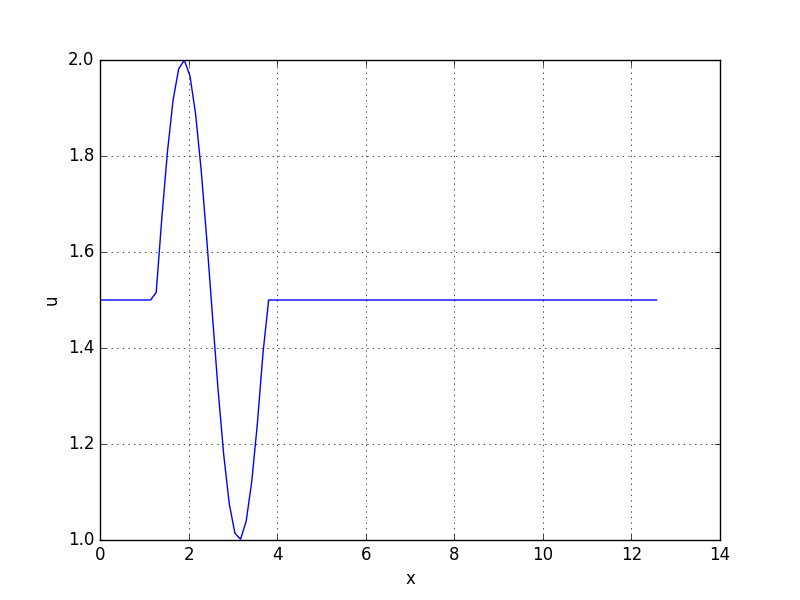
\includegraphics[scale=0.5]{hp-sol-n100-init}
	\caption{Initial condition}
\end{figure}
 

\begin{figure}[h!]
	\centering
	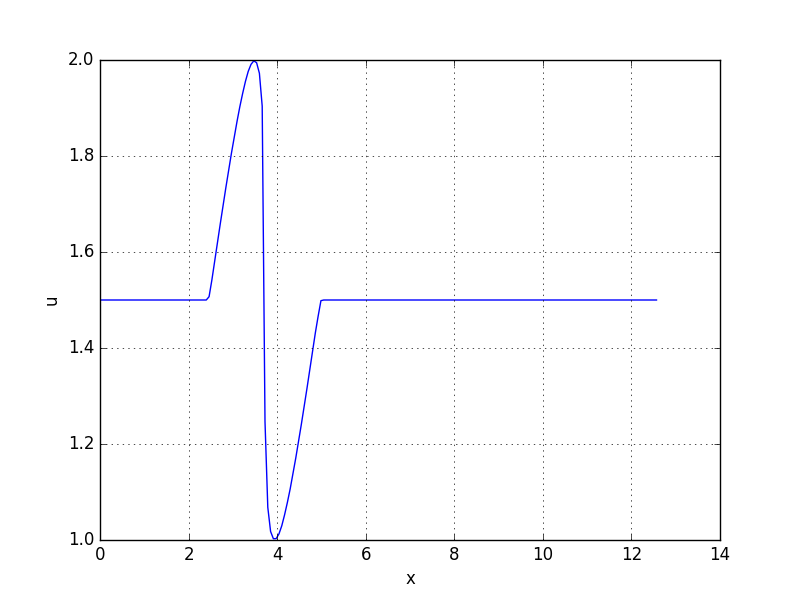
\includegraphics[scale=0.5]{hp-sol-t01}
	\caption{t = 0.1, before shock formation}
\end{figure}
 

\begin{figure}
	\centering
	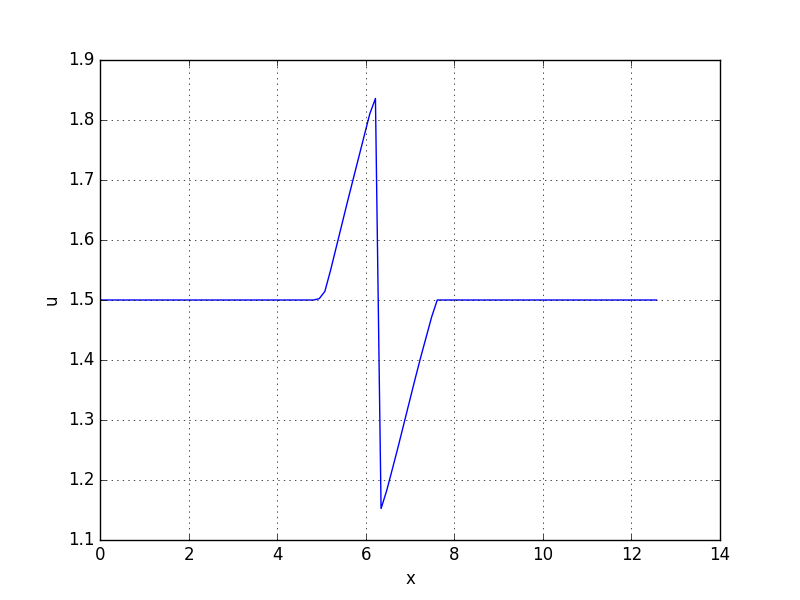
\includegraphics[scale=0.5]{hp-sol-n100-t25}
	\caption{t = 2.5, after shock formation}
\end{figure}
 
\begin{figure}
	\centering
	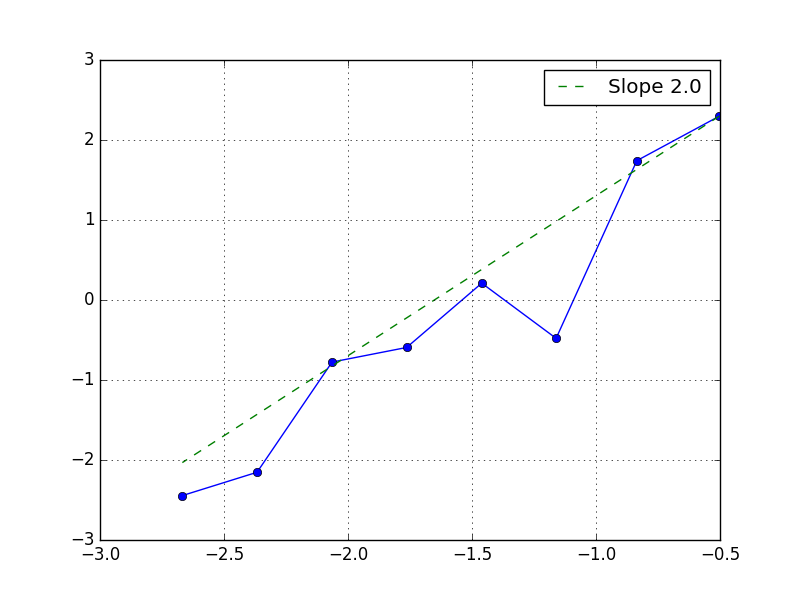
\includegraphics[scale=0.5]{hp-t25-grids8}
	\caption{Grid convergence for t = 2.5; the x axis is $\log_{10}||h||$, the y axis is $\log_{10}||u-u_{ref}||$}
\end{figure}
 
\begin{figure}
	\centering
	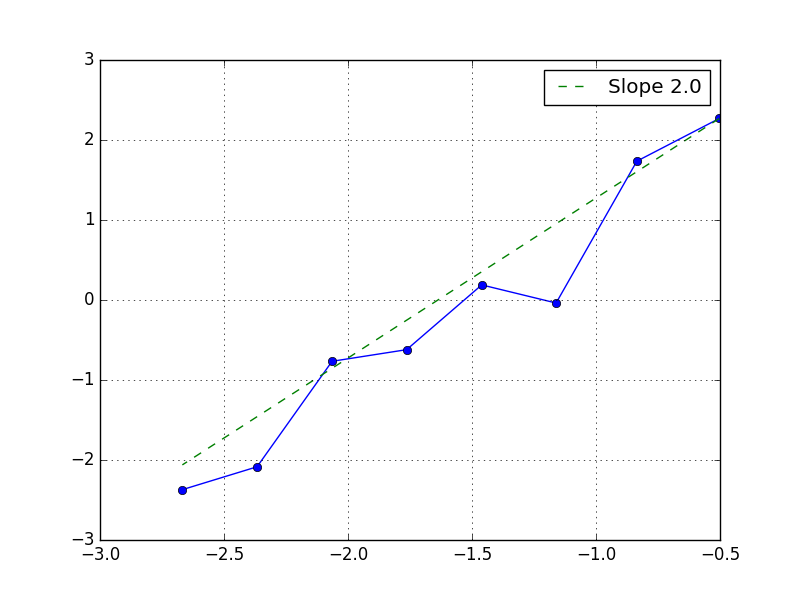
\includegraphics[scale=0.5]{hp-t25-nolocate}
	\caption{t = 2.5; no post-processing; the x axis is $\log_{10}||h||$, the y axis is $\log_{10}||u-u_{ref}||$}
\end{figure}
 
\FloatBarrier

\section{Conclusions and future work}
The particle method provides a way to achieve second-order accuracy for non-smooth solutions, at least for scalar conservation laws. An easy post-processing step is needed to maintain second-order accuracy in presence of shocks. In our opinion, this is the greatest strength of this method - a TVD second-order solution in presence of discontinuities.

However, extension to multi-dimensional problems and systems of conservation laws is not straightforward. Further, the fact that convergence, with increase in number of particles, need not be monotonic in general may also be an issue.

\subsection{Future work}

\subsubsection{Systems of conservation laws}
The derivative of the flux, $\bld{f}'(\bld{u})$, is now a matrix with $N$ eigenvalues. It is now not obvious what the speed of the particles should be taken as. Farjoun and Seibold propose one possible solution: use $N$ different sets of particles. But it is still not clear how the particles would interact. It is also a question whether TVD can be guaranteed for systems.

\subsubsection{Multidimensional problems}
In case of one-dimensional problems, we have `next' and `previous' particles. This is not the case for multi-dimensional problems. One could compute a Voronoi tessellation of the particles after each particle management step to get `neighbors' for each particle. The one-dimensional merge/insert could be applied to each pair of neighbors thus generated. This avenue could be pursued in order to solve multi-dimensional problems with not too much more complexity than the one-dimensional case.

Another possibly easily-resolvable issue is the computation of steady-state solutions when one exists.

\printbibliography

\end{document}